\chapter{Lý thuyết nhóm}

\begin{table}[htb]
    \caption{Thuật ngữ và ký hiệu}
    \begin{tabularx}{\textwidth}
        {|>{\raggedright\arraybackslash\hsize=0.2\textwidth}X|>{\raggedright\arraybackslash}X|}
        \hline
        \textbf{Ký hiệu} & \textbf{Ý nghĩa} \\ \hline\hline
        $\mathcal{S}_n$ & Nhóm hoán vị $n$ phần tử \\ \hline
        $\ker f$ & Hạt nhân (kernel) của ánh xạ $f$ \\ \hline
        $\Ima f$ & Ảnh (Image) của ánh xạ $f$ \\ \hline
        $\cong$ & Đẳng cấu nhóm (group isomorphism) \\ \hline
    \end{tabularx}
\end{table}

\section{Nhóm}

\subsection*{Nhóm và nhóm con}

\begin{definition}[Nhóm (Group)]
    Một tập hợp $G$ và toán tử 2 ngôi $\star$ trên $G$ tạo thành một nhóm nếu:
    \begin{enumerate}[noitemsep]
        \item Tồn tại phần tử $e \in G$ sao cho với mọi $g \in G$ thì $g \star e = e \star g = g$. Khi đó $e$ được gọi là \textbf{phần tử đơn vị} của $G$;
        \item Với mọi $g \in G$, tồn tại $g' \in G$ sao cho $g \star g' = g' \star g = e$. Khi đó $g'$ được gọi là \textbf{phần tử nghịch đảo} của $g$;
        \item Tính kết hợp: với mọi $a, b, c \in G$ thì $a \star (b \star c) = (a \star b) \star c$.
    \end{enumerate}
\end{definition}

\begin{definition}[Nhóm Abel]
    Nếu nhóm $G$ có thêm tính giao hoán, tức là với mọi $a, b \in G$ thì $a \star b = b \star a$ thì $G$ gọi là \textbf{nhóm giao hoán} hay \textbf{nhóm Abel}.
\end{definition}

\begin{example}
    Xét tập hợp số nguyên $\ZZ$ và phép cộng hai số nguyên.
    \begin{enumerate}[noitemsep]
        \item Phần tử đơn vị là 0 vì với mọi $a \in \ZZ$ thì $a + 0 = 0 + a = a$;
        \item Với mọi $a \in \ZZ$, phần tử nghịch đảo là $-a$ vì $a + (-a) = (-a) + a = 0$;
        \item Phép cộng số nguyên có tính kết hợp do đó thỏa mãn điều kiện về tính kết hợp.
    \end{enumerate}
    Như vậy $(\ZZ, +)$ tạo thành nhóm. Lưu ý do phép cộng hai số nguyên có tính giao hoán nên đây cũng là nhóm Abel.
\end{example}

\begin{example}
    Xét tập hợp số hữu tỉ khác 0 $\QQ^*$ và phép nhân 2 số hữu tỉ. Ta thấy do $a, b \in \QQ^*$ nên tích $a \cdot b$ cũng khác 0, do đó cũng thuộc $\QQ^*$.
    \begin{enumerate}
        \item Phần tử đơn vị là 1 vì với mọi $a \in \QQ^*$ thì $a \cdot 1 = 1 \cdot a = a$;
        \item Với mọi $a \in \QQ^*$, phần tử nghịch đảo là $\dfrac{1}{a}$ vì $a \cdot \dfrac{1}{a} = \dfrac{1}{a} \cdot a = 1$;
        \item Phép nhân hai số hữu tỉ có tính giao hoán do đó thỏa mãn điều kiện về tính kết hợp.
    \end{enumerate}
    Tương tự như nhóm $(\mathbb{Z, +})$, nhóm $(\QQ^*, \cdot)$ cũng là nhóm Abel.
\end{example}

\subsection*{Nhóm con}

\begin{definition}[Nhóm con (Subgroup)]
    Cho nhóm $(G, \star)$. Tập hợp $H \subset G$ được gọi là \textbf{nhóm con} của $G$ nếu với mọi $a, b \in H$ thì $a \star b \in H$
\end{definition}
 
Nghĩa là toán tử $\star$ đóng với các phần tử trong $H$.

\begin{example}
    Xét nhóm $(\ZZ, +)$ như trên. Ta xét tập con gồm các số chẵn của nó
    \[2\ZZ = \{\ldots, -4, -2, 0, 2, 4, \ldots\}\]

    Ta thấy rằng tổng 2 số chẵn vẫn là số chẵn, nghĩa là phép cộng số nguyên đóng trên $2\ZZ$.
    Do đó $(2\ZZ, +)$ là nhóm con của $(\ZZ, +)$.

    Như vậy mọi tập hợp có dạng $n \ZZ$ đều là nhóm con của $(\ZZ, +)$.
\end{example}

\subsection*{Coset}

\begin{definition}[Coset, \textit{lớp kề}]
    Cho nhóm $G$ và nhóm con $H$ của $G$.

    Coset trái của $H$ đối với phần tử $g \in G$ là tập hợp
    \[gH = \{gh : h \in H \}\]

    Tương tự, coset phải là tập hợp
    \[Hg = \{hg : h \in H \}\]
\end{definition}

Từ đây nếu không nói gì thêm ta ngầm hiểu là coset trái.

Ví dụ với nhóm con $2\ZZ$ của $\ZZ$, ta thấy rằng

\begin{enumerate}
    \item Nếu $g \in \ZZ$ là lẻ thì khi cộng với bất kì phần tử nào của $2\ZZ$ ta có số lẻ;
    \item Nếu $g \in \ZZ$ là chẵn thì khi cộng với bất kì phần tử nào của $2\ZZ$ ta có số chẵn.
\end{enumerate}

Nói cách khác, coset của $2\ZZ$ chia tập $\ZZ$ thành
\[0 + 2\ZZ = \{\ldots, -4, -2, 0, 2, 4, \ldots\}\]
 
\[1 + 2\ZZ = \{\ldots, -3, -1, 1, 3, \ldots \}\]

Rõ ràng hai coset trên rời nhau.

\begin{remark}
    Hai coset bất kì hoặc rời nhau, hoặc trùng nhau.
\end{remark}

\begin{proof}
    Nếu hai coset rời nhau thì không có gì phải nói. Ta chứng minh trường hợp còn lại.

    Giả sử $g_1 H \cap g_2 H \neq \emptyset$. Như vậy tồn tại $h_1, h_2 \in H$ mà $g_1 h_1 = g_2 h_2$.

    Do $h_1^{-1} \in H$, ta có $g_1 = g_2 h_2 h_1^{-1}$, nghĩa là $g_1 \in g_2 H$.

    Mà mọi phần tử trong $g_1 H$ có dạng $g_1 h$ nên $g_1 h = g_2 h_2 h_1^{-1} h$. Do $H$ là nhóm con của $G$ nên $h_2 h_1^{-1} h \in H$.
    Từ đó $g_1 H \subseteq g_2 H$. Tương tự ta cũng có $g_2 H \subseteq g_1 H$. Vậy $g_1 H = g_2 H$.
\end{proof}

\subsection*{Normal Subgroup}

\begin{definition}[Normal Subgroup, \textit{nhóm con chuẩn tắc}]
    Nhóm con $H$ của $G$ được gọi là \textbf{normal subgroup} nếu với mọi $g \in G$ ta có coset trái trùng với coset phải.
    \begin{equation*}
        gH = Hg \quad \text{ với mọi } g \in G
    \end{equation*}
\end{definition}

Nếu $H$ là normal subgroup của $G$ ta ký hiệu $H \triangleleft G$. Khi đó, với mọi
$a, b \in G$ thì $(a H) (b H) = (ab) H$.

\begin{definition}[Quotient Group, \textit{nhóm thương}]
    Với nhóm $G$ và normal subgroup của nó là $H$.
    Quotient Group được ký hiệu là $G / H$ và được định nghĩa là tập hợp các coset tương ứng với normal subgroup $H$.
    \[G / H = \{gH : g \in H \}\]

    Ta thấy rằng điều này chỉ xảy ra nếu $H$ là normal subgroup.
\end{definition}

Quotient Group còn được gọi là Factor Group - \textit{nhóm nhân tử}

\begin{example}
    Với nhóm $\ZZ$ và normal subgroup của nó là $2\ZZ$.
    Ta thấy $\ZZ / 2 \ZZ = \{0 + 2 \ZZ, 1 + 2 \ZZ\}$
\end{example}

\section{Nhóm hoán vị}

\subsection*{Nhóm hoán vị}

Xét tập hợp $\{ 1, 2, \ldots, n \}$. Ta gọi $\mathcal{S}_n$ là tập tất cả hoán vị của tập hợp trên. Như vậy $\mathcal{S}_n$ có $n!$ phần tử.

Nếu ta lấy hoán vị gốc là $(1, 2, \ldots n)$, mỗi hoán vị đều có thể được biểu diễn bằng hai hàng như sau
\begin{equation*}
    \sigma = \begin{pmatrix}
        1 & 2 & \ldots & n \\
        \sigma(1) & \sigma(2) & \ldots & \sigma(n)
    \end{pmatrix}
\end{equation*}

Ta định nghĩa toán tử trên $\mathcal{S}_n$. Với hai hoán vị $\sigma$ và $\tau$, hoán vị $\sigma \star \tau$ là vị trí của $\sigma$ theo $\tau$. Nói cách khác, nếu 
\begin{equation*}
    \sigma = \begin{pmatrix}
    1 & 2 & \ldots & n \\
    \sigma(1) & \sigma(2) & \ldots & \sigma(n)
\end{pmatrix}
\end{equation*}
và 
\begin{equation*}
    \tau = \begin{pmatrix}
    1 & 2 & \ldots & n \\
    \tau(1) & \tau(2) & \ldots & \tau(n)
\end{pmatrix}
\end{equation*}
thì 
\begin{equation*}
    \sigma \star \tau =
\begin{pmatrix}
    1 & 2 & \ldots & n \\
    \sigma(\tau(1)) & \sigma(\tau(2)) & \ldots & \sigma(\tau(n))   
\end{pmatrix}
\end{equation*}

Nhóm $\mathcal{S}_n$ và toán tử như trên tạo thành một nhóm và được gọi là
\textbf{nhóm hoán vị}.

\begin{example}
    Xét nhóm hoán vị $\mathcal{S}_5$. 
    
    Gọi $x = \begin{pmatrix}
        1 & 2 & 3 & 4 & 5 \\ 4 & 3 & 1 & 2 & 5
    \end{pmatrix}$ và
    $y = \begin{pmatrix}
        1 & 2 & 3 & 4 & 5 \\ 5 & 1 & 4 & 3 & 2
    \end{pmatrix}$. Khi đó, đặt $z = x \star y$ thì
    \begin{align*}
        & z(1) = x(y(1)) = x(5) = 5, \\
        & z(2) = x(y(2)) = x(1) = 4, \\
        & z(3) = x(y(3)) = x(4) = 2, \\
        & z(4) = x(y(4)) = x(3) = 1, \\ 
        & z(5) = x(y(5)) = x(2) = 3
    \end{align*}

    Như vậy $z = x \star y = \begin{pmatrix}
        1 & 2 & 3 & 4 & 5 \\ 5 & 4 & 2 & 1 & 3
    \end{pmatrix}$.
\end{example}

\begin{remark}
    Trong một hoán vị, khi biểu diễn trên hai hàng thì thứ tự viết không quan trọng, miễn là đảm bảo $i$ tương ứng với $\sigma(i)$ trên từng cột.
\end{remark}

\begin{example}
    Xét hoán vị $\sigma = \begin{pmatrix}
        1 & 2 & 3 & 4 & 5 \\ 4 & 3 & 1 & 2 & 5
    \end{pmatrix}$ thuộc $\mathcal{S}_5$.

    Ta có $\sigma(1) = 4$, $\sigma(2) = 3$, $\sigma(3) = 1$, $\sigma(4) = 2$
    và $\sigma(5) = 5$. Như vậy hai cách viết sau là giống nhau

    \begin{equation*}
        \sigma = 
        \begin{pmatrix}
            1 & 2 & 3 & 4 & 5 \\
            4 & 3 & 1 & 2 & 5
        \end{pmatrix} = 
        \begin{pmatrix}
            3 & 4 & 5 & 1 & 2 \\
            1 & 2 & 5 & 4 & 3
        \end{pmatrix}
    \end{equation*}
\end{example}

\subsection*{Chu trình độc lập}

Xét nhóm hoán vị $\mathcal{S}_n$ và hoán vị $\sigma$ thuộc $\mathcal{S}_n$.

Khi đó tồn tại các tập $\{ i_1, i_2, \ldots, i_k \} \subset \{1, 2, \ldots, n\}$
sao cho $\sigma(i_1) = i_2$, $\sigma(i_2) = i_3$, ..., $\sigma(i_{k-1})
= \sigma(i_k)$ và $\sigma(i_k) = i_1$.

\begin{example}
    Xét $\mathcal{S}_5$ và hoán vị $\sigma = \begin{pmatrix}
        1 & 2 & 3 & 4 & 5 \\ 5 & 1 & 4 & 3 & 2
    \end{pmatrix}$. 
    
    Ta thấy rằng $\sigma(1) = 5$, $\sigma(5) = 2$,
    $\sigma(2) = 1$. Như vậy ta có chu trình $1 \to 5 \to 2 \to 1$.

    Tương tự, $\sigma(3) = 4$ và $\sigma(4) = 3$. Như vậy ta
    có thêm chu trình $3 \to 4 \to 3$.

    Hai chu trình trên không chứa phần tử chung nên chúng được gọi là
    hai \textbf{chu trình độc lập}.
\end{example}

\begin{remark}
    Mọi hoán vị đều có thể viết được dưới dạng tích của các chu trình độc lập. \textbf{Chu trình có thể chứa một phần tử} ($\sigma(i) = i$).
\end{remark}

\begin{example}
    Hoán vị $\sigma = \begin{pmatrix}
        1 & 2 & 3 & 4 & 5 \\ 5 & 1 & 4 & 3 & 2
    \end{pmatrix}$ như trên thì ta có thể viết lại thành $\sigma = (1, 5, 2)(3, 4)$.
\end{example}

\begin{remark}
    Thứ tự của chu trình trong tích không quan trọng. Điều này dễ thấy vì các chu trình độc lập nhau, do đó dù  viết trước hay sau thì hoán vị vẫn nằm trong chu trình đó.
\end{remark}

Để giải thích rõ hơn, chúng ta có thể xem mỗi chu trình độc lập như một hoán vị, trong đó các phần tử không thuộc chu trình đứng yên. 

Ví dụ với chu trình $(1, 5, 2) = (1, 5, 2)(3)(4)$
ở trên tương đương với \[p_1 = \begin{pmatrix}
    1 & 2 & 3 & 4 & 5 \\ 5 & 1 & 3 & 4 & 2
\end{pmatrix}\] và với chu trình $(3, 4) = (3, 4)(1)(2)(5)$ tương đương với
\[p_2 = \begin{pmatrix}
    1 & 2 & 3 & 4 & 5 \\ 1 & 2 & 4 & 3 & 5
\end{pmatrix} = \begin{pmatrix}
    5 & 1 & 3 & 4 & 2 \\ 5 & 1 & 4 & 3 & 2
\end{pmatrix}\]

Do đó tích của chúng (hay toán tử trên nhóm hoán vị) sẽ cho ra kết quả hoán vị ban đầu.

\[\underbrace{\begin{pmatrix}
    1 & 2 & 3 & 4 & 5 \\ 5 & 1 & 4 & 3 & 2
\end{pmatrix}}_{\sigma} = \underbrace{\begin{pmatrix}
    1 & 2 & 3 & 4 & 5 \\ 5 & 1 & 3 & 4 & 2
\end{pmatrix}}_{p_1} \star \underbrace{\begin{pmatrix}
    5 & 1 & 3 & 4 & 2 \\ 5 & 1 & 4 & 3 & 2 
\end{pmatrix}}_{p_2}\]

\section{Group homomorphism}

\subsection*{Đồng cấu nhóm}

\begin{definition}[Đồng cấu nhóm]
    Xét hai nhóm $(G, \star)$ và $(H, *)$ và một ánh xạ $f: G \to H$.
    Ánh xạ $f$ được gọi là \textbf{đồng cấu} (hay \textbf{homomorphism}) nếu với mọi $g_1$, $g_2$ thuộc $G$ ta có $f(g_1 \star g_2) = f(g_1) * f(g_2)$.
\end{definition}

Do $g_1$, $g_2$ là các phần tử thuộc $G$ nên toán tử giữa chúng là $\star$. Trong khi đó $f(g_1)$, $f(g_2)$ là các phần tử thuộc $H$ nên toán tử giữa chúng là $*$.

\begin{remark}
    \begin{enumerate}
        \item Gọi $e_G$ là phần tử đơn vị của $G$ và $e_H$ là phần tử đơn
        vị của $H$. Khi đó $f(e_G) = e_H$
        \item Với mọi phần tử $g \in G$, nếu $g^{-1}$ là nghịch đảo của nó trong $G$ thì $f(g^{-1}) = f(g)^{-1}$
    \end{enumerate}
\end{remark}

\begin{proof}
    1. Nếu $e_G$ là phần tử đơn vị của $G$ thì với mọi $g \in G$ ta có $g \star e_G = e_G \star g = g$. Ta lấy $f$ cả 3 vế và theo định nghĩa homomorphism thu được $f(g \star e_G) = f(e_G \star g) = f(g) \Rightarrow f(g) * f(e_G) = f(e_G) * f(g) = f(g)$. Đẳng thức trên đúng với mọi $g \in G$ nên đúng với mọi $f(g)$, suy ra $f(e_G)$ là phần tử đơn vị trong nhóm $(H, *)$ và do đó $f(e_G) = e_H$
    
    2. Từ việc tìm ra phần tử đơn vị, ta cũng chứng minh được tính chất nghịch đảo trên.
\end{proof}

\subsection*{Các loại homomorphism}

Tương tự như ánh xạ, chúng ta có các loại homomorphism sau

\begin{definition}[Đơn cấu (Monomorphism)]
    Ánh xạ được gọi là \textbf{đơn cấu} (hay \textbf{monomorphism}) nếu nó là ánh xạ one-to-one (đơn ánh). Nói cách khác, với mọi $g_1 \neq g_2$ và $g_1$, $g_2 \in G$, thì $f(g_1) \neq f(g_2)$
\end{definition}

\begin{definition}[Toàn cấu (Epimorphism)]
    Ánh xạ được gọi là \textbf{toàn cấu} (hay \textbf{epimorphism}) nếu nó là ánh xạ onto (toàn ánh). Nói cách khác, với mọi $h \in H$ thì tồn tại $g \in G$ mà $f(g) = h$.
\end{definition}

\begin{definition}[Đẳng cấu (Isomorphism)]
    Ánh xạ được gọi là \textbf{đẳng cấu} (hay \textbf{isomorphism}) nếu nó là ánh xạ one-to-one 
    và onto (song ánh). Nói cách khác, ánh xạ này vừa là đơn cấu, vừa là toàn cấu.
\end{definition}

\begin{definition}[Tự đẳng cấu (Automorphism)]
    Ánh xạ được gọi là \textbf{tự đẳng cấu} (hay \textbf{automorphism}) nếu nó là song ánh từ nó lên chính nó. Ta ký hiệu tự đồng cấu nhóm $G$ là $\Aut(G)$.
\end{definition}

\subsection*{Hạt nhân và ảnh}

Xét một homomorphism $f$ từ nhóm $(G, \star)$ tới nhóm $(H, *)$. Ta nói

\begin{definition}[Hạt nhân (Kernel)]
    \textbf{Hạt nhân} (hay \textbf{kernel}) của $f$ là tập hợp các phần tử của $G$ cho ảnh là $e_H$, ký hiệu là $\ker f$. Nói cách khác
    \begin{equation}
        \ker f = \{ g \in G, f(g) = e_H \}
    \end{equation}
    Như vậy $\ker f$ là tập con của $G$.
\end{definition}

\begin{remark}
    $K = \ker f$ là normal subgroup của $G$.
\end{remark}

\begin{proof}
    Để chứng minh, ta thấy rằng theo định nghĩa homomorphism, với $g_1, g_2 \in K$ thì $f(g_1) = f(g_2) = e_H$.
    
    Ta có $f(g_1 \star g_2) = f(g_1) * f(g_2) = e_H * e_H = e_H$. Như vậy
    $g_1 \star g_2 \in K$ nên $K$ là nhóm con của $G$.
    
    Tiếp theo để chứng minh $K$ là normal subgroup, ta chứng minh
    $g K g^{-1} = K$ với mọi $g \in G$.

    Do $g K g^{-1} = \{ g \star k \star g^{-1} : k \in K \}$, lấy $f$ mỗi phần tử bên trong ta có 
    \[f(g \star k \star g^{-1}) = f(g) * f(k) * f(g^{-1}) = 
    f(g) * e_H * f(g^{-1}) = f(g) * f(g^{-1})\]
    mà theo tính chất của homomorphism thì $f(g^{-1}) = f(g)^{-1}$ nên $f(g \star k \star g^{-1}) = f(g) * f(g)^{-1} = e_H$ nên $g \star k \star g^{-1} \in K$ với mọi $g \in G$, với mọi $k \in K$. Do đó $g K g^{-1} = K$ và ta có điều phải chứng minh.
\end{proof}

\begin{definition}[Ảnh (Image)]
    \textbf{Ảnh} (hay \textbf{image}) của $f$ là tập hợp tất cả giá trị nhận được khi biến các phần tử thuộc $G$ thành phần tử thuộc $H$. Nói cách khác
    \begin{equation}
        \Ima f = \{ f(g), g \in G \}
    \end{equation}
    Như vậy $\Ima f$ là tập con của $H$.
\end{definition}

Dựa trên hai khái niệm này, chúng ta có một định lý quan trọng trong lý
thuyết nhóm là \textbf{Định lý thứ nhất về sự đẳng cấu} (First isomorphism theorem).

\begin{theorem}[First isomorphism theorem]
    Với hai nhóm $(G, \star)$ và $(H, *)$. Xét homomorphism $f: G \to H$. Khi đó $\Ima f$ đẳng cấu (isomorphism) với nhóm thương $G / \ker f$.
\end{theorem}

\begin{proof}
    Gọi $G$, $H$ là hai nhóm và homomorphism $f: G \to H$.
    Đặt $K = \ker f$. Ta xét biến đổi \[\theta:\,\Ima f \to G / K, f(g) \to g K \] với $g \in G$.

    Ta cần chứng minh biến đổi này là ánh xạ xác định (well-defined, nghĩa là tuân theo quy tắc ánh ánh xạ, mỗi phần tử tập nguồn biến thành \textbf{một và chỉ một} phần tử tập đích), là homomorphism, là đơn ánh và là toàn ánh.

    Đầu tiên ta chứng minh ánh xạ xác định. Giả sử ta có $g_1 K = g_2 K$, do $g_1$ và $g_2$ thuộc cùng coset nên $g_1^{-1} g_2 \in K$, hay $f(g_1^{-1} g_2) = e_H$.
    
    Với $f$ là homomorphism, ta có 
    \[f(g_1^{-1} g_2) = f(g_1^{-1}) f(g_2) = f(g_1)^{-1} f(g_2) = e_H\]
    Suy ra $f(g_1) = f(g_2)$. Như vậy nếu $f(g_1) = f(g_2)$ thì $\theta (f(g_1)) = \theta (f(g_2))$.

    Tiếp theo ta chứng minh $\theta$ là homomorphism. Do $K$ là normal subgroup của $G$ nên với mọi $g_1$, $g_2$ thuộc $G$ thì $g_1 g_2 K = (g_1 K) (g_2 K)$.

    Do $f(g_1 g_2) = f(g_1) f(g_2)$ nên 
    \[ \theta (f(g_1 g_2)) = g_1 g_2 K = (g_1 K) (g_2 K) = \theta (f(g_1)) 
    \theta (f(g_2)) \]
    Suy ra $\theta$ là homomorphism.

    Dễ thấy với mọi $g \in G$ ta đều tìm được $f(g)$ và $g K$ tương ứng. Do đó $\theta$ là toàn ánh.

    Để chứng minh $\theta$ là đơn ánh, giả sử $g_1 K = g_2 K$ ta có $g_1^{-1} g_2 \in K$ nên $f(g_1^{-1} g_2) = e_H$. Suy ra $f(g_1^{-1}) f(g_2) = e_H \Rightarrow f(g_1)^{-1} f(g_2) = e_H \Rightarrow f(g_1) = f(g_2)$. Như vậy $\theta$ là đơn ánh.

    Kết luận, $\theta$ là song ánh. Định lý thứ nhất về sự đẳng cấu được chứng minh.
\end{proof}

\section{Vành và trường}

\subsection*{Vành}

\begin{definition}[Vành (Ring)]
    Cho tập hợp $R$, trên đó ta định nghĩa hai toán tử \textbf{cộng} và \textbf{nhân}.

    Khi đó, $(R, +, \times)$ tạo thành \textbf{vành} (hay \textbf{ring}) nếu

    \begin{itemize}
        \item $(R, +)$ là nhóm Abel;
        \item $(R, \times)$ có tính kết hợp với phép nhân. Với mọi $a, b, c \in R$ thì $a \times (b \times c) = (a \times b) \times c$;
        \item Tính phân phối của phép cộng và phép nhân. Với mọi $a, b, c \in R$ thì $(a + b) \times c = a \times c + b \times c$.
    \end{itemize}
\end{definition}

Tóm lại, $(R, +, \times)$ là vành nếu nó là nhóm Abel đối với phép cộng và có tính kết hợp với phép nhân.

\textbf{Lưu ý}. Phép nhân ở đây không nhất thiết có phần tử đơn vị, hay phần tử nghịch đảo như trong định nghĩa nhóm. Trong trường hợp này $(R, \times)$ gọi là semigroup (nửa nhóm).

\begin{definition}[Vành với đơn vị (Ring with identity)] 
    Nếu có phần tử $1_R \neq 0_R \in R$ sao cho với mọi $r \in R$ ta đều có
    \begin{equation*}
        1_R \times r = r \times 1_R = r
    \end{equation*}
    thì $1_R$ được gọi là phần tử đơn vị đối với phép nhân.
\end{definition}

Ta thường ký hiệu $0_R$ là phần tử đơn vị của phép cộng $(R, +)$ và gọi là \textbf{phần tử trung hòa}.
Khi đó phần tử nghịch đảo của phép cộng gọi là \textbf{phần tử đối} và được ký hiệu là $-a$, chỉ phần tử đối của phần tử $a$.

Ta ký hiệu $1_R$ là \textbf{phần tử đơn vị} đối với phép nhân $(R, \times)$.

Từ phần tử đơn vị đối với phép nhân ta có khái niệm đặc số (characteristic) của vành với đơn vị.

\begin{definition}[Đặc số (Characteristic)]
    Xét trường $R$ với phần tử đơn vị là $1$ và phần tử trung hòa là 0. Số dương $p$ nhỏ nhất sao cho
    \begin{equation*}
        \underbar{1 + 1 + \ldots + 1 + 1}_{n \text{ lần}} = 0
    \end{equation*}
    được gọi là \textbf{đặc số} (hay \textbf{characteristic}) của $R$.
\end{definition}

\begin{definition}[Vành giao hoán (Commutative Ring)]
    Nếu ta có tính giao hoán đối với phép nhân, nghĩa là với mọi $a, b \in $ đều thỏa
    \begin{equation*}
        a \times b = b \times a
    \end{equation*}
    thì ta nói là vành giao hoán.
\end{definition}

\subsection*{Trường}

\begin{definition}[Trường (Field)]
    Cho tập hợp $F$ và hai toán tử hai ngôi trên $F$ là phép cộng $+$ và phép nhân $\times$. Khi đó $(F, +, \times)$ là \textbf{trường} (hay \textbf{field}) nếu
    \begin{itemize}
        \item $(F, +, \times)$ là vành giao hoán với đơn vị
        \item Với mọi phần tử $f \neq 0_F$, tồn tại nghịch đảo $f^{-1}$ của $f$ đối với phép nhân, nghĩa là $f \times f^{-1} = f^{-1} \times f = 1_F$
    \end{itemize}
\end{definition}

Nói cách khác, $(F, \times)$ là nhóm Abel. Trên trường ta thực hiện được bốn phép tính cộng, trừ, nhân, chia.

\begin{example}
    Các tập hợp sau với phép cộng và nhân là trường.
    \begin{enumerate}
        \item Tập hợp số thực $\RR$;
        \item Tập hợp các số phức $\CC$;
        \item Tập hợp các số dạng $a + b \sqrt{2}$ với $a, b \in \QQ$.
    \end{enumerate}
\end{example}

Những trường trên được gọi là \textbf{trường vô hạn} vì có vô số phần tử.

Ngược lại, chúng ta cũng có các \textbf{trường hữu hạn}.

\subsection*{Trường hữu hạn}

\subsubsection*{Trường hữu hạn modulo nguyên tố}

Cho $p$ là số nguyên tố. Khi đó tập hợp các số dư khi chia cho $p$ cùng với phép cộng và nhân modulo $p$ tạo thành trường.

\begin{proof}
    Xét tập hợp các số dư khi chia cho $p$ là $S = \{0, 1, \ldots, p-2, p-1\}$.

    Ta thấy rằng với mọi $a, b \in S$ thì $a + b \pmod p$ và $a \cdot b \pmod p$ đều thuộc $S$.

    \begin{itemize}
        \item Vì $0 + a = a + 0 = a \pmod p$ với mọi $a \in S$ nên $0$ là phần tử đơn vị của phép cộng.
        \item Với mọi $a \in S$, ta có $(p-a) + a = a + (p-a) \equiv 0 \pmod p$ nên phần tử nghịch đảo của $a$ 
        đối với phép cộng là $p-a \in S$.
        \item Phép cộng modulo có tính kết hợp
        \item Phép cộng modulo có tính giao hoán
    \end{itemize}
    Như vậy $(S, +)$ là nhóm Abel.

    Tiếp theo, ta thấy rằng phép cộng và nhân có tính phân phối trên modulo.
    Đồng thời phép nhân modulo cũng có tính kết hợp. Do đó $(S, +, \cdot)$ là vành.

    \begin{itemize}
        \item Phần tử đơn vị của phép nhân là 1
        \item Phép nhân modulo có tính giao hoán
        \item Do mọi phần tử thuộc $S$ đều nguyên tố cùng nhau với $p$ nên luôn tồn tại nghịch đảo của phần tử khác 0 trong $S$
    \end{itemize}
    Kết luận: $(S, +, \cdot)$ là trường.
\end{proof}

Ta thường ký hiệu trường này là $GF(p)$ (GF là viết tắt của Galois Field để tưởng nhớ người có đóng góp quan trọng trong lý thuyết nhóm).

\subsubsection*{Trường hữu hạn modulo đa thức}

Xét các đa thức với hệ số nguyên
\begin{equation*}
    f(x) = a_n x^n + a_{n-1} x^{n-1} + \ldots + a_2 x^2 + a_1 x + a_0
\end{equation*}

Ta thấy rằng phép cộng và nhân hai đa thức tạo thành một vành giao hoán với đơn vị (đa thức $f(x) \equiv 1$).

Thêm nữa vành này có vô số phần tử. Ta cần một phương án để số phần tử là hữu hạn, và đồng thời là trường.

Với $p$ là số nguyên tố và $n$ là số nguyên dương. Mình xét các đa thức có bậc tối đa là $n-1$ với hệ số nằm trong tập hợp các số dư khi chia cho $p$. Như vậy mình có $p^n$ đa thức như vậy.

\begin{example}
    Với $p=3$ và $n=2$. Khi đó các đa thức có thể có là
    $0, 1, 2, x, x+1, x+2, 2x, 2x+1, 2x+2$
\end{example}

Tương tự với việc modulo cho một số nguyên tố, ở đây mình xét phép cộng và nhân trên modulo một đa thức tối giản (irreducible polynomial) có bậc $n$ (vì khi modulo một đa thức bậc bất kì cho đa thức bậc $n$ ta có đa thức bậc nhỏ hơn $n$). 

Đồng thời hệ số của đa thức từ phép cộng và nhân cũng được modulo $p$ (nằm trong $GF(p)$).

Với trường hợp $p=3$ và $n=2$ ở trên mình có thể chọn đa thức modulo là $m(x) = x^2 + 2x + 2$. Khi đó bảng phép nhân (phép cộng khá đơn giản nên mình không viết) 2 đa thức bậc nhỏ hơn 2 trong modulo $m(x)$ là bảng \ref{gf_mult_3}

\begin{table}[htb]
    \centering
    \begin{subtable}[h]{\textwidth}
        \centering
        \begin{tabular}{|c|c|c|c|c|c|}
            \hline
            & 0 & 1 & 2 & $x$ & $x+1$ \\
            \hline
            0 & 0 & 0 & 0 & 0 & 0 \\
            \hline
            1 & 0 & 1 & 2 & $x$ & $x+1$ \\
            \hline
            2 & 0 & 2 & 1 & $2x$ & $2x+2$\\
            \hline
            $x$ & 0 & $2x$ & $x+1$ & $2x$ & $2x+1$ \\
            \hline
            $x+1$ & 0 & $x+1$ & $2x+2$ & $2x+1$ & 2\\
            \hline
            $x+2$ & 0 & $x+2$ & $2x+1$ & 1 & $x$ \\
            \hline
            $2x$ & 0 & $2x$ & $x$ & $2x+2$ & $x+2$ \\
            \hline
            $2x+1$ & 0 & $2x+1$ & $x+2$ & 2 & $2x$ \\
            \hline
            $2x+2$ & 0 & $2x+2$ & $x+1$ & $x+2$ & 1 \\
            \hline
        \end{tabular}
        \caption{Nửa đầu bảng nhân}
    \end{subtable}
    
    \begin{subtable}[h]{\textwidth}
        \centering
        \begin{tabular}{|c|c|c|c|c|}
            \hline
            & $x+2$ & $2x$ & $2x+1$ & $2x+2$ \\
            \hline
            0 & 0 & 0 & 0 & 0 \\
            \hline
            1 & $x+2$ & $2x$ & $2x+1$ & $2x+2$ \\
            \hline
            2 & $2x+1$ & $x$ & $x+2$ & $x+1$ \\
            \hline
            $x$ & 1 & $2x+2$ & 2 & $x+2$ \\
            \hline
            $x+1$ & $x$ & $x+2$ & $2x$ & 1 \\
            \hline
            $x+2$ & $2x+2$ & 2 & $x+1$ & $2x$ \\
            \hline
            $2x$ & 2 & $x+1$ & 1 & $2x+1$ \\
            \hline
            $2x+1$ & $x+1$ & 1 & $2x+2$ & $x$ \\
            \hline
            $2x+2$ & $2x$ & $2x+1$ & $x$ & 2 \\
            \hline
        \end{tabular}
        \caption{Nửa sau bảng nhân}
    \end{subtable}
    \caption{Bảng nhân trên $GF(3^2)$}
    \label{gf_mult_3}
\end{table}

Ta thấy rằng bảng phép nhân đối xứng qua đường chéo chính. Điều này chứng tỏ phép nhân có tính giao hoán. Thêm nữa ở mỗi hàng hoặc cột khác 0 đều có 9 phần tử khác nhau.

\subsection*{Ideal}

\begin{definition}[Ideal]
    Xét vành $(R, +, \times)$. Một tập con $I$ của $R$ được gọi là \textbf{ideal trái} nếu
    \begin{itemize}
        \item $(I, +)$ là nhóm con của $(R, +)$;
        \item với mọi $r \in R$, với mọi $x \in I$ thì $rx \in I$.
    \end{itemize}
\end{definition}

Ta định nghĩa tương tự với ideal phải, khi đó $xr \in I$. Từ đây về sau nếu không nói gì thêm nghĩa là mình xét ideal trái.

\begin{definition}[Ideal chính (Principal Ideal)]
    Nếu $I = aR$ với $a$ là phần tử nào đó trong $R$ thì $I$ được gọi là \textbf{principal ideal}.
\end{definition}

Nói cách khác, nếu có một phần tử trong $R$ "sinh" ra được $I$ thì $I$ là principal.

\begin{definition}[Ideal cực đại (Maximal Ideal)]
    Nếu $I$ là một ideal của $R$ và không tồn tại tập con $I'$ mà $I \subset I' \subset R$ (tập con thực thụ) thì $I$ được gọi là \textbf{maximal ideal}.
\end{definition}

\begin{corollary}
    Xét vành số nguyên $\ZZ$. Khi đó mọi ideal của $\ZZ$ đều là principal.
\end{corollary}

\begin{proof}
    Giả sử ideal $I$ của $\ZZ$ có phần tử dương nhỏ nhất là $n$.
    Theo định nghĩa của ideal thì với mọi $q \in \ZZ$ ta có 
    $qn \in I$.

    Nếu phần tử $a \in I$, theo phép chia Euclid ta có $a = qn + r$
    với $0 \leq r < n$, mà $a \in I$ và $qn \in I$ nên $r = a - qn \in I$.
    Tuy nhiên phần tử dương nhỏ nhất thuộc $I$ là $n$, do đó $r = 0$.

    Nói cách khác mọi phần tử $a \in I$ đều có dạng $qn$ với $q \in \ZZ$.

    Vậy mọi ideal đều là principal.
\end{proof}

\begin{corollary}
    Ideal $I$ của $\ZZ$ là maximal khi và chỉ khi $I = n\ZZ$ với $n$ là số nguyên tố.
\end{corollary}

\begin{proof}
    Ta chứng minh chiều thuận, chiều ngược tương tự. Sử dụng phản chứng,
    ta giả sử $n$ là hợp số. Khi đó $n = n_1 n_2$ ($n_1 \geq n_2 > 1$).

    Khi đó $n \ZZ \subset n_1 \ZZ \subset \ZZ$, suy ra ideal không phải
    maximal. Ta có điều phải chứng minh.
\end{proof}

\begin{theorem}
    Gọi $R$ là vành giao hoán với đơn vị. Khi đó, nếu $I$ là ideal của $R$ thì $R / I$ là trường khi và chỉ khi $I$ là maximal ideal.
\end{theorem}

\begin{proof}
    Ta chứng minh điều kiện cần và điều kiện đủ.

    \underline{Điều kiện cần}. Ta có $I$ là maximal ideal. Ta thấy rằng
    $a + I \neq 0 \Leftrightarrow a \not\in I$. Vì nếu $a \in I$ thì 
    tồn tại $-a \in I$. Theo định nghĩa vành thì $a R$ cũng là ideal
    nên $I + a R$ là ideal, mà $a \not\in I$ và $a \in I + a R$ suy ra
    $I \subset I + a R$. Ta lại có $I$ là maximal nên $I + aR = R$, 
    do đó tồn tại $n \in I$ và $b \in R$ sao cho $n + ab = 1$. Tóm 
    lại là tồn tại nghịch đảo của phép nhân, do đó $R / I$ là trường.
    
    \underline{Điều kiện đủ}. Với $R / I$ là trường. Ta giả sử $I$ không là
    maximal ideal. Khi đó tồn tại $I'$ sao cho $I \subset I' \subset R$.
    Khi đó tồn tại phần tử $a \in I'$ và $a \not\in I$ mà $a + I \neq 0$.
    Do đó $(a + I) (b + I) = 1 + I$ suy ra tồn tại $n \in I \subset I'$ 
    sao cho $a b = 1 + n$. Do $a, b \in I'$ nên $1 \in I'$, từ đó
    $1 \in R$ nên $I'$ không phải maximal.
\end{proof}

\begin{example}
    Xét tập hợp $\ZZ$ là vành giao hoán với đơn vị. Khi đó nếu $n$ là số nguyên tố thì $n \ZZ$ là maximal ideal (đã chứng minh ở trên). Do đó tập $\ZZ / n\ZZ$ là trường hữu hạn modulo nguyên tố gồm các phần tử $\{ 0, 1, \ldots, p-1 \}$.
\end{example}

\section{Tác động nhóm}

Tác động nhóm (Group Action) cho phép chúng ta đếm những cấu hình tổ hợp mà việc vét cạn rồi loại bỏ sẽ tốn nhiều công sức cũng như sai sót.

\subsection*{Tác động nhóm}

Cho tập hợp $M$ và nhóm $G$. Ta nói $G$ \textbf{tác động trái} lên $M$ với ánh xạ:
\[\alpha: G \times M \rightarrow M\]
thỏa mãn 2 tiên đề sau:

\begin{itemize}
    \item Identity: $\alpha (e, m) = m$ với mọi $m \in M$ và $e$ là phần tử đơn vị của $G$;
    \item Compatibility: $\alpha (g, \alpha (h, m)) = \alpha (g h, x)$.
\end{itemize}

Ta thường ký hiệu $\alpha (g, m)$ bởi $g(m)$ hay thậm chí đơn giản hơn là $gm$. Ký hiệu $gm$ sẽ được sử dụng từ đây về sau.

Khi đó 2 tiên đề trên tương đương với:

\begin{itemize}
    \item Identity: $e m = m$ với mọi $m \in M$;
    \item Compatibility: $g(hm) = (gh)m$ với mọi $m \in M$ và $g, h \in G$.
\end{itemize}

\begin{definition}[Stabilizer - \textit{nhóm con ổn đinh}]
    Với phần tử $m \in M$ cho trước, tập hợp các phần tử $g \in G$ mà $gm = m$ được gọi là \textbf{stabilizer} của nhóm $G$. Ta ký hiệu
    \[G_m = \{ g \in G : gm = m \}\]
\end{definition}

\begin{definition}[Orbit - \textit{quỹ đạo}]
    Orbit của phần tử $m \in M$ là tập hợp
    \[G(m) = \{gm : g \in G\}\]
\end{definition}

\begin{remark}
    Hai orbit của hai phần tử bất kì hoặc rời nhau, hoặc trùng nhau.
\end{remark}

\begin{proof}
    Giả sử ta có $m_1, m_2 \in M$ mà $G(m_1) \cap G(m_2) \neq \emptyset$.

    Khi đó tồn tại $g_1, g_2 \in G$ để $g_1 m_1 = g_2 m_2$. Suy ra $m_1 = g_1^{-1} g_2 m_2$.

    Mà mọi phần tử trong $G(m_1)$ có dạng $g m_1$ nên $g m_1 = g g_1^{-1} g_2 m_2$ nên $G(m_1) \subseteq G(m_2)$.

    Chứng minh tương tự ta cũng có $G(m_2) \subseteq G(m_1)$ nên $G(m_1) \equiv G(m_2)$.
\end{proof}

\begin{corollary}
    Tập hợp $M$ là giao của các orbit rời nhau. Giả sử ta có $t$ orbit rời nhau $G(m_1), G(m_2), \ldots, G(m_t)$ thì
    \[M = G(m_1) \cup G(m_2) \cup \ldots \cup G(m_t)\]
\end{corollary}

\begin{example}
    Cho nhóm $\mathcal{S}_3$ có 6 phần tử $(1)(2)(3)$, $(1)(2,3)$, $(2)(1,3)$, $(3)(1,2)$, $(1,2,3)$, $(1,3,2)$.

    Xét tập hợp $M = \{1, 2, 3\}$. Khi đó, xét từng hoán vị trên, ta có:
    \[G_1 = \{(1)(2)(3), (1)(2,3)\}\]
    và
    \[G(1) = \{ 1, 2, 3 \}\]
\end{example}

Ta nhận thấy $G(1) = G(2) = G(3)$, và $\lvert G \rvert = 6 = \lvert G_1 \rvert \cdot \lvert G(1) \rvert$

Hay nói cách khác, $\lvert G(m) \rvert = [G: G_m]$ với $G_m$ là stabilizer của phần tử $m$ và $[G: G_m]$ là subgroup index của $G_m \subset G$, và bằng $\dfrac{\lvert G \rvert}{\lvert G_m \rvert}$ nếu là nhóm hữu hạn.

\begin{definition}
    Hai phần tử $m, n \in M$ được gọi là \textbf{có quan hệ} với nhau dưới tác động của nhóm $G$ nếu tồn tại phần tử $g \in G$ sao cho $m = g n$.
    Ta ký hiệu là $m \tilde{G} n$.
\end{definition}

\begin{remark}
    Quan hệ được định nghĩa như trên là quan hệ tương đương.
\end{remark}

\begin{proof}
    Để chứng minh một quan hệ là tương đương, ta cần chứng minh tính phản xạ, đối xứng và bắc cầu.

    Đối với tính phản xạ, mọi vector đều có quan hệ với chính nó qua phần tử đơn vị $e \in G$.

    Đối với tính đối xứng, nếu $m$ có quan hệ với $n$ thì tồn tại $g \in G$ sao cho $m = gn$. Theo tính chất nhóm thì tồn tại phần tử $g^{-1}$ là nghịch đảo của $g$ trong $G$. Do đó $g^{-1} m = n$. Nói cách khác $n$ cũng có quan hệ với $m$. Như vậy ta có tính đối xứng.

    Đối với tính bắc cầu, nếu $m$ có quan hệ với $n$ thì tồn tại $g_1 \in G$ sao cho $m = g_1 n$. Tiếp theo, nếu $n$ có quan hệ với $p$ thì tồn tại $g_2 \in G$ sao cho $n = g_2 p$. Suy ra $m = g_1 n = g_1 (g_2 p) = (g_1 g_2) p$. Do $g_1, g_2 \in G$ nên $g_1 g_2 \in G$. Như vậy $m$ cũng có quan hệ với $p$ nên quan hệ có tính bắc cầu.

    Vậy quan hệ được định nghĩa như trên là quan hệ tương đương.
\end{proof}

\subsection*{Bổ đề Burnside}

Các trạng thái khác nhau của tập hợp $M$ là \textbf{tương đương} nhau nếu chúng nằm trong cùng lớp tương đương dưới tác động của nhóm $G$.

Các ví dụ về bổ đề Burnside và định lý Polya được tham khảo tại \cite{Tarannikov}.

\begin{lemma}[Bổ đề Burnside]
    Với nhóm $G$ tác động lên tập hợp $M$, ta có:
    \begin{equation*}
        t_G = \frac{1}{\lvert G \rvert} \sum_{g \in G} \lvert M^g \rvert
    \end{equation*}
    trong đó:
    \begin{itemize}
        \item  $t_G$ là số lớp tương đương của tập $M$ dưới tác động của nhóm $G$;
        \item $\lvert M^g \rvert$ là số điểm bất động của tập $M$ dưới tác động của phần tử $g$, nghĩa là $M^g = \{ m \in M : gm = m\}$.
    \end{itemize}
\end{lemma}

\subsection*{Bài toán tô màu bốn đỉnh tứ diện}

Cho hình tứ diện đều. Ta tô bốn đỉnh của nó bằng ba màu xanh, đỏ, vàng. Hỏi có bao nhiêu cách tô như vậy?

Ta cần lưu ý một điều, hai cách tô là tương đương nhau (giống nhau) nếu tồn tại một phép quay các đỉnh biến cách tô này thành cách tô kia.

\begin{figure}[ht]
    \centering
    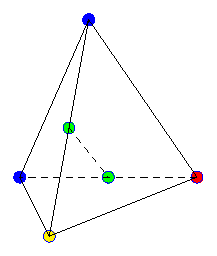
\includegraphics[page=1]{figures/tetrahedron.pdf}
    \includegraphics[page=2]{figures/tetrahedron.pdf}
    \caption{Phép quay trục tạo bởi trung điểm hai cạnh đối nhau}
\end{figure}

Như hình trên ta thấy nếu chọn trục quay là đường thẳng nối trung điểm 2 cạnh đối diện (2 điểm xanh lá) thì đỉnh trên và đỉnh dưới đổi chỗ cho nhau (xanh và vàng), đỉnh trái và đỉnh phải đổi chỗ cho nhau (xanh và đỏ).

Ta giải bài này như sau:

Đầu tiên ta đánh số các đỉnh của tứ diện (như hình)

\begin{figure}[htb]
    \centering
    \includegraphics[page=3]{figures/tetrahedron.pdf}
    \caption{Đánh số hình}
\end{figure}

Ta có 3 trường hợp biến đổi sau:

\underline{Trường hợp 1}. Giữ nguyên 1 đỉnh và trục quay là đường thẳng đi qua đỉnh đó và tâm của mặt đối diện.

\begin{figure}[htb]
    \centering
    \includegraphics[page=4]{figures/tetrahedron.pdf}
    \caption{Trường hợp 1}
\end{figure}

Khi đó phép quay (ngược chiều đồng hồ) tương ứng hoán vị $(1)(2,3,4)$ (quay 60 độ) và $(1)(2,4,3)$ (quay 120 độ).

Do ta chọn 1 đỉnh cố định thì ta có 4 cách chọn, và với mỗi cách chọn đỉnh cố định ta có thể quay 2 cách nên ta có tổng là 8 hoán vị.

\underline{Trường hợp 2}. Ta chọn trung điểm 2 cạnh đối nhau và nối lại thành trục quay như hình trong ví dụ. Khi đó tương ứng với hoán vị $(1,4)(2,3)$.

Ta có $\dfrac{C^2_4}{2!} = 3$ hoán vị.

\underline{Trường hợp 3}. Hoán vị đồng nhất $(1)(2)(3)(4)$.

Tóm lại, tập hợp $M$ ở đây là tập hợp 4 đỉnh của tứ diện, và nhóm tác động lên $M$ là nhóm con 12 phần tử của $\mathcal{S}_4$.

Như vậy, ví dụ với hoán vị $(1)(2,3,4)$, nếu ta muốn sau phép quay giữ nguyên trạng thái (hay nói cách khác là tìm $M^g$) thì ta
tô màu đỉnh 1 tùy ý, đỉnh 2-3-4 chung màu (cũng tùy ý).

Suy ra ta có $3 \cdot 3$ cách tô. Tương tự với các hoán vị dạng $(1,4)(2,3)$.

Như vậy $t_G = \dfrac{1}{12}(1 \cdot 3^4 + 8 \cdot 3^2 + 3 \cdot 3^2) = 15$ cách tô màu khác nhau.

Tổng quát, nếu có $k$ màu thì số lớp tương đương là
\[t_G = \dfrac{1}{12}\left(1 \cdot k^4 + 8 \cdot k^2 + 3 \cdot k^2\right) = \dfrac{1}{12}(k^4 + 11 k^2)\]

\subsection*{Tác động nhóm lên vector}

Xét nhóm $G$ và không gian vector $\FF_2^n$, $n \in \NN$. Khi đó hai vector $\bm{x}$ và $\bm{y}$ thuộc $\FF_2^n$ được gọi là \textbf{quan hệ với nhau} nếu tồn tại $g \in G$ mà $\bm{x} = g \bm{y}$.

Ví dụ, xét nhóm hoán vị $\mathcal{S}_3$. Giả sử các vector trong $\FF_2^3$ có dạng \[ \bm{x} = (x_1, x_2, x_3) \in \FF_2^3. \] 

Khi đó vector $(1, 0, 0)$ có quan hệ với $(0, 0, 1)$ với hoán vị $(1, 3)(2)$. Cụ thể là $(x_1, x_2, x_3) \xrightarrow{(1, 3)(2)} (x_3, x_2, x_1)$.

Tương tự, vector $(1, 0, 0)$ cũng có quan hệ với $(0, 1, 0)$ với hoán vị $(1, 2)(3)$. Thêm nữa, vector $(1, 0, 0)$ có quan hệ với chính nó qua hoán vị đồng nhất $(1)(2)(3)$.

Trong môn toán rời rạc ta đã biết, nếu một tập có quan hệ tương đương thì ta có thể phân các phần tử của tập đó vào các lớp tương đương rời nhau. Nghĩa là nếu hai phần tử có quan hệ với nhau thì vào cùng một lớp tương đương. Từ phần trên ta đã biết rằng dưới tác động của nhóm, các phần tử trong tập hợp bất kì sẽ phân bổ thành các lớp tương đương.

Câu hỏi đặt ra là, có bao nhiêu lớp tương đương như vậy?

Để giải quyết vấn đề này ta sử dụng bổ đề Burnside.

Nhóm $\mathcal{S}_3$ có các hoán vị \[ \mathcal{S}_3 = \{ (1)(2)(3), (1, 2)(3), (1, 3)(2), (2, 3)(1), (1, 3, 2), (1, 2, 3) \} \]

Lần lượt xét từng hoán vị. Đầu tiên, với $(1)(2)(3)$ thì các phần tử trong vector đứng yên. Do đó dưới tác động của hoán vị này, $x_1$ biến thành $x_1$, $x_2$ biến thành $x_2$ và $x_3$ biến thành $x_3$. Số cách chọn cho mỗi $x_i$ là 2 nên theo quy tắc nhân ta có $2^3 = 8$ cách.

Tiếp theo, với hoán vị $(1, 2)(3)$ thì $x_1 \to x_2$, $x_2 \to x_1$ và $x_3 \to x_3$. Do đó $x_1$ và $x_2$ có cùng giá trị nên có 2 cách chọn, $x_3$ cũng có 2 cách chọn nên tổng số cách là $2 \cdot 2 = 4$. Hoán vị $(1, 3)(2)$ và $(2, 3)(1)$ tương tự.

Với hoán vị $(1, 2, 3)$ thì $x_1 \to x_2$, $x_2 \to x_3$ và $x_3 \to x_1$ nên $x_1 = x_2 = x_3$, có 2 cách chọn trong trường hợp này. Hoán vị $(1, 3, 2)$ tương tự.

Như vậy, theo bổ đề Burnside, số lớp tương đương các vector trong $\FF_2^3$ là \[ t(\mathcal{S}_3) = \frac{1}{6} (1 \cdot 2^3 + 3 \cdot 2^2 + 2 \cdot 2) = 4 \]

Thật vậy, ta có thể chia các vector thành 4 lớp tương đương là $\{ 000 \}$, $\{ 001, 010, 011 \}$, $\{ 011, 101, 110 \}$, $\{ 111 \}$.

Ngoài nhóm $\mathcal{S}_3$ ra còn các nhóm khác cũng tác động lên các vector. Một số nhóm hay được sử dụng là:

\begin{enumerate}
    \item Nhóm general linear: gồm các ma trận khả nghịch $n \times n$ trên $\FF_2$. Tác động nhóm lúc này là phép nhân ma trận $\bm{A} \in GL(n, 2)$ với vector $\bm{x} \in \FF_2^n$, hay $\bm{A} \cdot \bm{x}$.
    \item Nhóm general affine: gồm các ma trận khả nghịch $n \times n$ trên $\FF_2$ và vector bất kì trong $\FF_2^n$. Tác động nhóm lúc này là biến đổi affine $\bm{A} \cdot \bm{x} + \bm{b}$ với $\bm{A} \in GL(n, 2)$ và $\bm{b} \in \FF_2^n$.
\end{enumerate}

%Cần nhắc lại một chút, số lượng phần tử của nhóm $GL(n, 2)$ là \[ (2^n - 1) \cdot (2^n - 2) \cdots (2^n - 2^{n-1}) \]

%Khi $n = 3$ thì $\lvert GL(3, 2) \rvert = (2^3 - 1) \cdot (2^3 - 2) \cdot (2^3 - 4) = 168$ ma trận.

\subsection*{Tác động nhóm lên hàm boolean}

Ta tiếp tục xét nhóm $G$ và không gian vector $\FF_2^n$, $n \in \NN$. Khi đó hai hàm boolean $n$ biến $f(x_1, \ldots, x_n)$ và $g(x_1, \ldots, x_n)$ được gọi là \textbf{quan hệ với nhau} nếu tồn tại $g \in G$ mà $g(\bm{x}) = f(g \bm{x})$ với mọi $\bm{x} \in \FF_2^n$.

Ta cũng xét hoán vị $\mathcal{S}_3$. Ta cũng lần lượt xét các phần tử của nhóm.

Đặt $f_0, f_1, \ldots, f_7$ lần lượt là các giá trị hàm $f$ với các vector $\bm{x} \in \FF_2^3$.

Đầu tiên, với $(1)(2)(3)$, ta có bảng chuyển vector như hình \ref{burnside:first}.

\begin{figure}[ht]
    \centering
    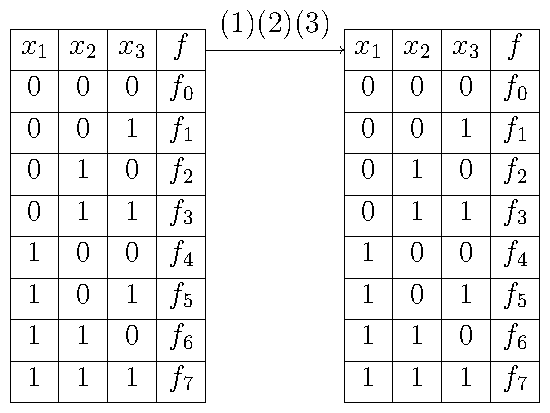
\includegraphics[page=1]{figures/burnside.pdf}
    \caption{Hoán vị $(1)(2)(3)$}
    \label{burnside:first}
\end{figure}

Ta thấy rằng $f_0 \to f_0$, $f_1 \to f_1$, ..., $f_7 \to f_7$ nên có 8 chu trình. Vậy số lượng cách chọn là $2^8$.

Tiếp theo, xét các hoán vị dạng $(1)(2, 3)$, ta có bảng chuyển vector như hình \ref{burnside:second}.

\begin{figure}[ht]
    \centering
    \includegraphics[page=2]{figures/burnside.pdf}
    \caption{Hoán vị $(1)(2, 3)$}
    \label{burnside:second}
\end{figure}

Ta thấy rằng $f_0 \to f_0$, $f_1 \to f_2 \to f_1$, $f_3 \to f_3$, $f_4 \to f_4$, $f_5 \to f_6 \to f_5$, $f_7 \to f_7$. Ở đây có 6 chu trình nên số cách chọn là $2^6$.

Tiếp theo ta xét các hoán vị dạng $(1, 2, 3)$ (hình \ref{burnside:third}).

\begin{figure}[ht]
    \centering
    \includegraphics[page=3]{figures/burnside.pdf}
    \caption{Hoán vị $(1, 2, 3)$}
    \label{burnside:third}
\end{figure}

Ta thấy rằng $f_0 \to f_0$, $f_1 \to f_2 \to f_4 \to f_1$, $f_3 \to f_6 \to f_5 \to f_3$, $f_7 \to f_7$ nên ở đây có 4 chu trình. Số cách chọn là $2^4$.

Như vậy theo bổ đề Burnside, số lớp hàm bool tương đương dưới tác động của nhóm $\mathcal{S}_3$ là \[ t (\mathcal{S}_3) = \dfrac{1}{6}(2^8 + 3 \cdot 2^6 + 2 \cdot 2^4) = 80. \]

\subsection*{Định lý Polya}

Với mỗi hoán vị trong tập $G$, ta viết dưới dạng các chu trình độc lập
\begin{equation*}
    \underbrace{(g_1) (g_2) \ldots (g_{t_{1}})}_{t_1} \underbrace{(g_{j_1} g_{j_2}) (g_{j_3} g_{j_4})}_{t_2} \ldots
\end{equation*}

Nếu ta viết hoán vị dưới dạng các chu trình rời nhau, ta gọi

\begin{table}
    \begin{tabularx}{\textwidth}
        {>{\raggedright\arraybackslash\hsize=0.1\textwidth}X >{\raggedright\arraybackslash}X}
        $t_1$ & là số chu trình có độ dài 1 \\
        $t_2$ & là số chu trình có độ dài 2 \\
        $\ldots$ & tương tự \\
        $t_n$ & là số chu trình có độ dài $n$
    \end{tabularx}
\end{table}

Khi đó, \textbf{cycle index} (hay \textbf{chỉ số chu trình}) của hoán vị ứng các biến $z_1, z_2, \ldots, z_n$ là
\begin{equation*}
    I_g (z_1, z_2, ,\ldots, z_n) = z_1^{t_1} z_2^{t_2} \ldots z_n^{t_n}
\end{equation*}

\begin{example}
Xét hoán vị $(1,2,3)(4)(5)(6,7) \in \mathcal{S}_7$

Ta có hai chu trình độ dài 1, một chu trình độ dài 2 và một chu trình độ dài 3 và không có chu trình độ dài 4, 5, 6, 7.

Do đó chỉ số chu trình là $I_g (z_1, z_2, z_3) = z_1^2 z_2^1 z_3^1$.

\end{example}

\begin{remark}
    Bất kì hoán vị nào thuộc $\mathcal{S}_n$ đều thỏa $1 \cdot t_1 + 2 \cdot t_2 + \ldots + n \cdot t_n = n$.
\end{remark}

\begin{definition}[Cyclic index - \textit{chỉ số chu trình}]
    \textbf{Chỉ số chu trình} của nhóm G là
    \[P_G (z_1, z_2, \ldots, z_n) = \frac{1}{G}\sum_{g \in G} I_g (z_1, z_2, \ldots, z_n)\]
\end{definition}

Nhìn lại ví dụ về tứ diện bên trên, các đỉnh nằm trong cùng chu trình cần được tô cùng màu. Từ đó ta có chỉ số chu trình
\begin{equation*}
    P_G(z_1, z_2, z_3) = \frac{1}{12}\big(z_1^4 + 8 z_1 z_3 + 3 z_2^2\big)
\end{equation*}

Cho mỗi $z_i = 3$ ta có kết quả phép tính theo bổ đề Burnside.

Định lý Polya là một mở rộng cho bổ đề Burnside, cho phép chúng ta đếm số lớp tương đương thỏa mãn điều kiện nhất định (về số lượng phần tử).

Ví dụ với hình tứ diện như trên nhưng ta thêm điều kiện tô hai đỉnh màu vàng, một đỉnh màu đỏ và một đỉnh màu xanh.

Ta ký hiệu tập $R$ là tập hợp các trạng thái có thể nhận của mỗi phần tử $m \in M$.
\[R = \{r_1, r_2, \ldots, r_c \}\]
Ở ví dụ trên thì $R = \{\text{đỏ}, \text{xanh}, \text{vàng}\}$.

Ta thay mỗi $z_i$ trong chỉ số chu trình bằng tổng $\displaystyle{\sum_{r \in R} r^i}$.

\begin{example}
    Giả sử ta tô màu 4 đỉnh tứ diện với 2 màu $R = \{r_1, r_2\}$.

    Với $z_1$ ta thay bằng $r_1 + r_2$

    Với $z_2$ ta thay bằng $r_1^2 + r_2^2$

    Với $z_3$ ta thay bằng $r_1^3 + r_2^3$

    Khi đó $P_G$ tương đương với
    \[\frac{1}{12}\big[(r_1 + r_2)^4 + 8 \cdot (r_1 + r_2)(r_1^3 + r_2^3) + 3 \cdot (r_1^2 + r_2^2)^2\big]\]
    Ta khai triển $P_G$ (lưu ý là ở đây không có tính giao hoán phép nhân)
    \begin{align*}
        (r_1 + r_2)^4 = & r_1 r_1 r_1 r_1 + r_1 r_1 r_1 r_2 + r_1 r_1 r_2 r_1 + r_1 r_1 r_2 r_2 \\
        + & r_1 r_2 r_1 r_1 + r_1 r_2 r_1 r_2 + r_1 r_2 r_2 r_1 + r_1 r_2 r_2 r_2 \\
        + & r_2 r_1 r_1 r_1 + r_2 r_1 r_1 r_2 + r_2 r_1 r_2 r_1 + r_2 r_1 r_2 r_2 \\
        + & r_2 r_2 r_1 r_1 + r_2 r_2 r_1 r_2 + r_2 r_2 r_2 r_1 + r_2 r_2 r_2 r_2
    \end{align*}
    Mình thấy rằng có 16 cấu hình khác nhau tương ứng 16 cách tô 2 màu cho 4 đỉnh. Tương tự
    \begin{align*}
        (r_1 + r_2) (r_1^3 + r_2^3) & = r_1^4 + r_1 r_2^3 + r_2 r_1^3 + r_2^4 \\
        & = r_1 r_1 r_1 r_1 + r_1 r_2 r_2 r_2 + r_2 r_1 r_1 r_1 + r_2 r_2 r_2 r_2
    \end{align*}
    và cuối cùng
    \begin{align*}
        (r_1^2 + r_2^2)^2 & = r_1^4 + r_1^2 r_2^2 + r_2^2 r_1^2 + r_2^4 \\
        & = r_1 r_1 r_1 r_1 + r_1 r_1 r_2 r_2 + r_2 r_2 r_1 r_1 + r_2 r_2 r_2 r_2
    \end{align*}

    Việc không có tính giao hoán với phép nhân làm biểu thức cồng kềnh và phức tạp.
    Do đó mình thêm một tập hợp $W$ là vành giao hoán, và xét ánh xạ $w: R \mapsto W$ với $w(r_i) = w_i$.

    Khi đó nếu thay $r_i$ bởi $w_i$ vào bên trên biểu thức sẽ rất đẹp
    \[P_G(w_1, w_2) = \frac{1}{12} \big[(w_1 + w_2)^4 + 8 (w_1 + w_2) (w_1^3 + w_2^3) + 3 (w_1^2 + w_2^2)^2\big]\]

    Khai triển và thu gọn ta có
    \begin{align*}
    P_G(w_1, w_2) & = \frac{1}{12} \big[12 w_1^4 + 12 w_1^3 w_2 + 12 w_1^2 w_2^2 + 12 w_1 w_2^3 + 12 w_2^4\big] \\
    & = w_1^4 + w_1^3 w_2 + w_1^2 w_2^2 + w_1 w_2^3 + w_2^4
    \end{align*}

    Ở đây, định lý Polya nói rằng, số mũ của $w_i$ thể hiện số lượng phần tử của tập $M$ nhận giá trị $r_i$,
    và hệ số trước mỗi toán hạng là số lớp tương đương tương ứng với số lượng phần tử của tập $M$ nhận các giá trị $r_i$.

    Nói cách khác:
    \begin{itemize}
        \item có 1 lớp tương đương mà 4 đỉnh nhận màu $r_1$;
        \item có 1 lớp tương đương mà 3 đỉnh nhận màu $r_1$ và 1 đỉnh nhận màu $r_2$;
        \item có 1 lớp tương đương mà 2 đỉnh nhận màu $r_1$ và 2 đỉnh nhận màu $r_2$;
        \item có 1 lớp tương đương mà 1 đỉnh nhận màu $r_1$ và 3 đỉnh nhận màu $r_2$;
        \item có 1 lớp tương đương mà 4 đỉnh nhận màu $r_2$.
    \end{itemize}
\end{example}

Quay lại vấn đề tô bốn đỉnh tứ diện với ba màu xanh, đỏ, vàng. Tìm số cách tô hai đỉnh màu vàng, một đỉnh màu đỏ và một đỉnh màu xanh.

Đặt $w(\text{vàng}) = x$, $w(\text{đỏ}) = y$ và $w(\text{xanh}) = z$.

Ta có
\[P_G = \frac{1}{12} \big[(x + y + z)^4 + 8 \cdot (x + y + z) (x^3 + y^3 + z^3) + 3 \cdot (x^2 + y^2 + z^2)^2\big]\]

Như vậy đề bài tương ứng việc tìm hệ số của hạng tử $x^2 yz$ trong biểu thức trên. Kết quả là 1.